
\documentclass{exam}

\usepackage{graphicx}
\usepackage[fleqn]{amsmath}
\usepackage{unitsdef} 
\usepackage{cancel}
\usepackage{float}
\usepackage{mdwlist}
\usepackage{booktabs}
\usepackage{cancel}
\usepackage{polynom}
\usepackage{caption}
\usepackage{fullpage}
\usepackage{enumerate}
% \usepackage{parskip}

% \newcommand{\degree}{\ensuremath{^\circ}} 
\everymath{\displaystyle}

\newunit{\inch}{in}
\newunit{\foot}{ft}
\newunit{\cemtimeter}{cm}

% \begin{figure}[H]
%   \centering
%   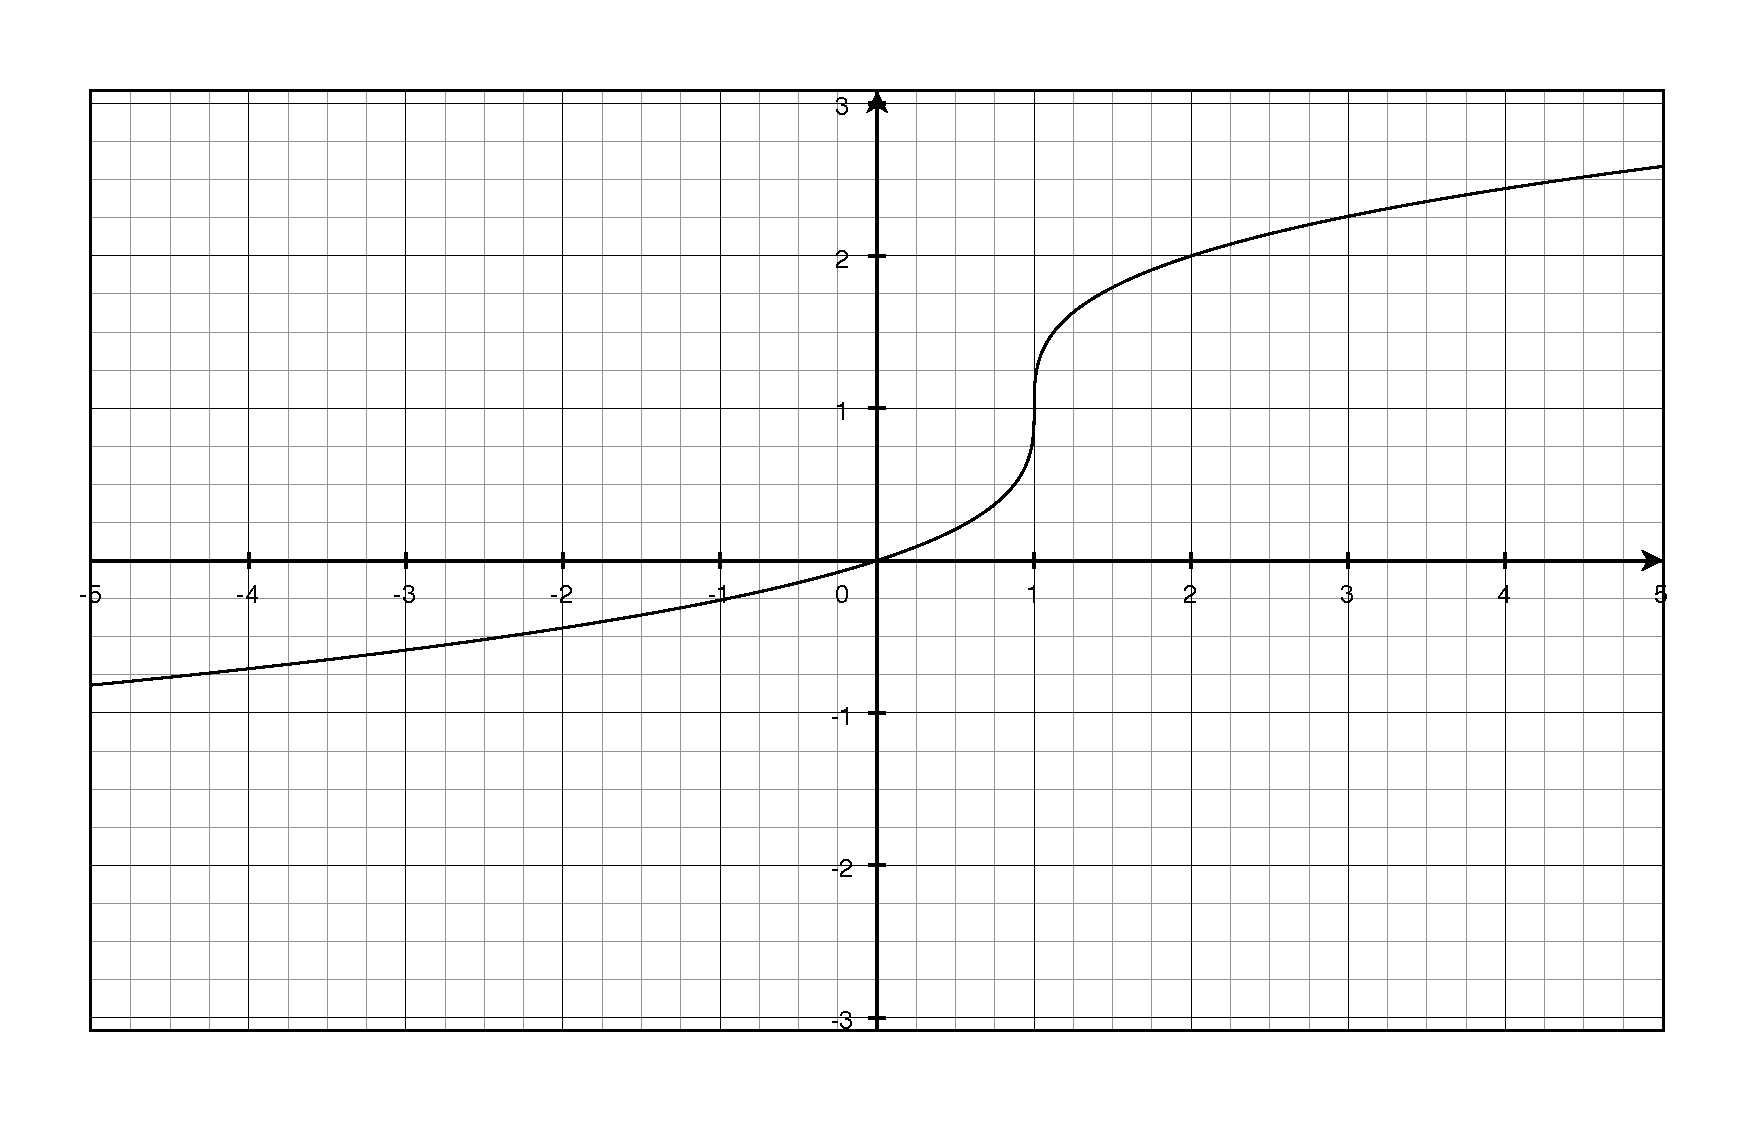
\includegraphics[scale=.3]{question7.eps}
%   \caption*{Question 7}
% \end{figure}

% \begin{tabular}{cc}
% \toprule
% period & amplitude \\
% \midrule
%   $\pi$ & $2$ \\
% \bottomrule
% \end{tabular}

\printanswers

\ifprintanswers 
\usepackage{2in1, lscape} 
\fi

\title{Math 263B \\ Homework Eleven}
\date{November 29, 2012}

\begin{document}

\maketitle

\section{Homework}

\begin{itemize*}
  \item Read Section 7.2
  \item pp 357-359: 7, 10, 13, 15-17, 21-22, 25-26, 35-38
\end{itemize*}

%% \ifprintanswers
%% \pagebreak
%% \fi

\section{Extra Credit}
page 359, problem 43
\ifprintanswers
\begin{solution}
This integral is the area between the function and the x-axis
\[
  \int_0^1 f(x) \, \mathrm{d}x
\]

This integral is the area between the function and the y-axis
\[
  \int_0^1 f^{-1}(y) \, \mathrm{d}y
\]

The total area for the two integrals must be 1 since they add up to fill a 1x1 square.  Since the first integral is 2/5,
the second integral must be 3/5. 

\end{solution}

\section{Section 7.2}

\begin{description}
\item[7]
\begin{align*}
  f(x)  &= -x^5 - x^3 \\
  f'(x) &= -5x^4 - 3x^2 \\
        &= -(5x^4 + 3x^2) \\
\end{align*}

Since the quantity inside the parentheses is always greater than or equal to zero, $f'$ is always less than or equal to
zero.

\item[10]
\begin{align*}
  f(x)  &= \cot x \\
        &= \frac{\cos x}{\sin x} \\
  f'(x) &= \frac{\sin x (- \sin x) - \cos x \cdot \cos x}{\sin^2 x} \\
        &= -\frac{1}{\sin^2 x} \\
        &= -\csc^2 x \\
\end{align*}

Since $\csc^2 x > 0$ in the interval $\left(0, \frac{\pi}{2} \right)$, $f'(x) < 0$ in this interval.

\item[13]
\begin{align*}
  f(x)  &= \int_0^x \sqrt{t^4 + t^2 + 10}\, \mathrm{d}t \\
  f'(x) &= D_x \int_0^x \sqrt{t^4 + t^2 + 10}\, \mathrm{d}t \\
        &= \sqrt{x^4 + x^2 + 10} \\
\end{align*}

$f'(x) > 0$ for all $x$.

\item[15]
solve for $y$ in terms of $x$
\begin{align*}
  y &= x + 1 \\
  x &= y - 1 \\
\end{align*}
replace $y$ with $x$ in the result:
\[
  f^{-1}(x) = x - 1
\]
verify:
\begin{align*}
  f(f^{-1}(x)) &= (x - 1) + 1 = x \\
  f^{-1}(f(x)) &= (x + 1) - 1 = x \\
\end{align*}

\item[16]
solve for $y$ in terms of $x$
\begin{align*}
  y &= - \frac{x}{3} + 1 \\
  x &= 3 - 3y \\
\end{align*}
replace $y$ with $x$ in the result:
\[
  f^{-1}(x) = 3 - 3x \\
\]
verify:
\begin{align*}
  f(f^{-1}(x))  &= - \frac{3 - 3x}{3} + 1 = x \\
  f^{-1}(f(x)) &= 3 - 3 \left( - \frac{x}{3} + 1 \right) = x \\  
\end{align*}

\item[17]
solve for $y$ in terms of $x$
\begin{align*}
  y &= \sqrt{x + 1} \\
  x &= y^2 - 1 \\
\end{align*}
replace $y$ with $x$ in the result:
\[
  f^{-1}(x) = x^2 - 1 \\
\]
verify:
\begin{align*}
  f(f^{-1}(x))  &= \sqrt{(x^2 - 1) + 1} = x \\
  f^{-1}(f(x)) &= \left(\sqrt{x + 1}\right)^2 - 1 = x \\  
\end{align*}

%% \item[18]
%% Notice that for this problem, $y \leq 0$ for any $x$ in the domain.  So the domain for $f^{-1}(x)$ is $(-\infty, 0]$.

%% solve for $y$ in terms of $x$
%% \begin{align*}
%%   y &= - \sqrt{1 - x} \\
%%   x &= 1 - y^2 \\
%% \end{align*}
%% replace $y$ with $x$ in the result:
%% \[
%%   f^{-1}(x) = 1 - x^2 \\
%% \]
%% verify:
%% \begin{align*}
%%   f(f^{-1}(x))  &= - \sqrt{1 - (1 - x^2)} = -x \\
%%   f^{-1}(f(x)) &= 1 - (-\sqrt{1 - x})^2 = -x \\  
%% \end{align*}

%% Since $x$ is always negative, 

\item[21]
solve for $y$ in terms of $x$
\begin{align*}
  y &= 4x^2 \\
  x &= \frac{\sqrt{y}}{2} \\
\end{align*}
replace $y$ with $x$ in the result:
\[
  f^{-1}(x) = \frac{\sqrt{x}}{2} \\
\]
verify:
\begin{align*}
  f(f^{-1}(x))  &= 4 \cdot \left( \frac{\sqrt{x}}{2} \right)^2 = x \\
  f^{-1}(f(x)) &= \frac{\sqrt{4x^2}}{2} = x \\  
\end{align*}

\item[22]
solve for $y$ in terms of $x$
\begin{align*}
  y &= (x - 3)^2 \\
  x &= 3 + \sqrt{y} \\
\end{align*}
replace $y$ with $x$ in the result:
\[
  f^{-1}(x) = 3 + \sqrt{x} \\
\]
verify:
\begin{align*}
  f(f^{-1}(x)) &= (3 + \sqrt{x} - 3)^2 = x \\
  f^{-1}(f(x)) &= 3 + \sqrt{(x - 3)^2} = x \\  
\end{align*}

\item[25]
solve for $y$ in terms of $x$
\begin{align*}
  y &= \frac{x - 1}{x + 1} \\
  x &= \frac{y + 1}{1 - y} \\
\end{align*}
replace $y$ with $x$ in the result:
\[
  f^{-1}(x) = \frac{x + 1}{1 - x} \\
\]
verify:
\begin{align*}
  f(f^{-1}(x)) &= \frac{\left(\cfrac{x + 1}{1 - x} - 1\right)}{\left(\cfrac{x + 1}{1 - x} + 1 \right)} = x \\
  f^{-1}(f(x)) &= \frac{\left(\cfrac{x - 1}{x + 1} + 1 \right)}{\left(1 - \cfrac{x - 1}{x + 1} \right)} = x \\  
\end{align*}

\item[26]
solve for $y$ in terms of $x$
\begin{align*}
  y &= \left( \frac{x - 1}{x + 1} \right)^3 \\
  x &= \frac{\sqrt[3]{y} + 1}{1 - \sqrt[3]{y}} \\
\end{align*}
replace $y$ with $x$ in the result:
\[
  f^{-1}(x) = \frac{\sqrt[3]{x} + 1}{1 - \sqrt[3]{x}}
\]
verify:
\begin{align*}
  f(f^{-1}(x)) &= \left(\frac{ \left(\cfrac{\sqrt[3]{x} + 1}{1 - \sqrt[3]{x}} - 1 \right)}
                            { \left(\cfrac{\sqrt[3]{x} + 1}{1 - \sqrt[3]{x}} + 1 \right)} \right)^3 = x \\
  f^{-1}(f(x)) &= \frac{\left( \sqrt[3]{\left( \cfrac{x - 1}{x + 1} \right)^3} + 1 \right)}
                        {\left(1 - \sqrt[3]{\left( \cfrac{x - 1}{x + 1} \right)^3} \right)} = x \\  
\end{align*}

\item[35]
find $x$ for $y = 2$:
\begin{align*}
  2 &= 3x^5 + x - 2 \\
  3x^5 + x - 4 &= 0 \\
  x &= 1 \\
\end{align*}

find the derivative:
\begin{align*}
  f(x) &= 3x^5 + x - 2 \\
  f'(x) &= 15x^4 + 1 \\
\end{align*}

find $(f^{-1})'(2)$:
\begin{align*}
  (f^{-1})'(2) &= \frac{1}{f'(1)} \\
    &= \frac{1}{15 \cdot 1^4 + 1} \\
    &= \frac{1}{16} \\
\end{align*}

\item[36]
find $x$ for $y = 2$:
\begin{align*}
  2 &= x^5 + 5x - 4 \\
  x &= 1 \\
\end{align*}
find the derivative:
\begin{align*}
  f(x) &= x^5 + 5x - 4 \\
  f'(x) &= 5x^4 + 5 \\
\end{align*}
find $(f^{-1})'(2)$:
\begin{align*}
  (f^{-1})'(2) &= \frac{1}{f'(1)} \\
    &= \frac{1}{5 \cdot 1^4 + 5} \\
    &= \frac{1}{10} \\
\end{align*}

\item[37]
find $x$ for $y = 2$:
\begin{align*}
  2 &= 2 \tan x \\
  x &= \frac{\pi}{4} \\
\end{align*}
find the derivative:
\begin{align*}
  f(x) &= 2 \tan x \\
  f'(x) &= 2 \sec^2 x \\
\end{align*}
find $(f^{-1})'(2)$:
\begin{align*}
  (f^{-1})'(2) &= \frac{1}{f'(1)} \\
    &= \frac{1}{\left( 2 \sec^2 \cfrac{\pi}{4} \right)} \\
    &= \frac{1}{\left( 2 \cdot \left( \sqrt{2} \right)^2 \right)} \\
    &= \frac{1}{4} \\
\end{align*}

\item[38]
find $x$ for $y = 2$:
\begin{align*}
  2 &= \sqrt{x + 1} \\
  x &= 3 \\
\end{align*}
find the derivative:
\begin{align*}
  f(x) &= (x + 1)^{1/2} \\
  f'(x) &= \frac{1}{2 \sqrt{x + 1}} \\
\end{align*}
find $(f^{-1})'(2)$:
\begin{align*}
  (f^{-1})'(2) &= \frac{1}{f'(3)} \\
    &= 2 \sqrt{3 + 1} \\
    &= 4 \\
\end{align*}



\end{description}

\else

\vspace{8 cm} {\em No observation will cause one to be ejected from acceptable mainstream company more immediately than
  pointing out that what the U.S. Government is doing is ``terrorism'' by definition \ldots That's because using
  terrorist threats (or civilian-destroying violence) for political gain, or to keep a population in fear, is something
  that only other people do---but never the United States---even when it's as plain as day (as it is here) that the
  U.S. Government is doing exactly that.}

\hspace{0.5 cm} --Glenn Greenwald

%% {\em Some writers have so confounded society with government, as to leave little or no distinction between them; whereas
%%   they are not only different, but have different origins. Society is produced by our wants, and government by our
%%   wickedness; the former promotes our happiness POSITIVELY by uniting our affections, the latter NEGATIVELY by
%%   restraining our vices. The one encourages intercourse, the other creates distinctions. The first a patron, the last a
%%   punisher.} --Thomas Paine

%% Value judgments are destructive to our proper business, which is curiosity and awareness. -- John Cage
\fi

\end{document}

